\documentclass[12pt, oneside]{revtex4}   	% use "amsart" instead of "article" for AMSLaTeX format
%\usepackage{geometry}                		% See geometry.pdf to learn the layout options. There are lots.
%\geometry{letterpaper}                   		% ... or a4paper or a5paper or ... 
%\geometry{landscape}                		% Activate for for rotated page geometry
%\usepackage[parfill]{parskip}    		% Activate to begin paragraphs with an empty line rather than an indent
\usepackage{graphicx}				% Use pdf, png, jpg, or eps§ with pdflatex; use eps in DVI mode
								% TeX will automatically convert eps --> pdf in pdflatex		
\usepackage{amssymb}
\usepackage{mathtools}
\usepackage{subcaption}
\captionsetup{compatibility=false}
\usepackage{float}
\usepackage{wrapfig}
\usepackage{setspace}
\begin{document}
\title{Children's Learned Associations with Voice: Investigating Children's Speech Perception and Socialization}
\author{Nicholas P. Moores \\ Departments of Linguistics and Psychology, Stanford University}
\date{5 June 2015}							% Activate to display a given date or no date

\maketitle
%\section{}
%\subsection{}
\section{Abstract}
Examining the processing of spoken words enables us to investigate children's burgeoning ability to extract social information in the speech stream. The speech signal contains not only phonemic information necessary for word recognition but abundant indexical information about the talker, including talker gender (Perry, Ohde, \& Ashmead, 2001; Goldinger, 1998; Johnson et al., 1999; Johnson, 2006). A growing body of work has begun to investigate the effects of listeners' associations between talkers' social identity and phonetic cues in talkers' voices, demonstrating that by adulthood listeners use talker information to make social inferences about a talker's likely behavior (Van Berkum et al., 2008), especially when listeners expect talker identity to be useful or find it to be a reliable cue (Creel, Aslin, \& Tanenhaus, 2008). Recent work suggests that children use acoustic cues to talker identity to constrain comprehension of spoken language (Creel, 2012), though the way in which children learn to integrate social knowledge with information from voice remains poorly understood. In this paper, we test the hypothesis that children are able to disambiguate between objects with gendered associations (a men's pair of gloves and a women's pair of gloves, say) based on talker voice. We explore children's use of talker-specific information to infer speaker meaning through an experiment in which children interact with a web page on an iPad. Over 24 trials, children ages 3-5 were shown series of four images and asked by talkers to find one of the objects by clicking on it. During half of the trials, children heard a male talker's voice, and during the other half they heard a female talker's voice. In addition, half of the trials were non-competitor trials where there was only one image of the referent (hearing a man's voice and seeing a man's glove, say). The other half were competitor trials in which the target image competed with a variant which would stereotypically belong to a speaker of the other gender (hearing a man's voice but choosing between both a man's glove and a woman's glove). Children's reaction time was measured from the onset of the utterance of the target word to their click on an image, and their choice of image was recorded. Our data suggest that by age 5, children regularly integrate phonetically-cued social information with their knowledge of speaker characteristics to guide their interpretations of speaker meaning in a real world paradigm. From age 3 to 5, their ability to associate voice types with speaker gender and speaker intention increases significantly. Our results suggest that children make use of socially-nuanced speaker-specific acoustic information by a young age, and reveal their robust understanding of gender stereotypes that guide their daily interactions with interlocutors and may bear on their linguistic and social development.

\section{Introduction}
\subsection{Social Encoding and the Speech Stream}
The speech stream is rich with phonetic variation that cues information about sounds and words, and information necessary for conveying and perceiving speaker identity (Perry, et al., 2001; Goldinger, 1998; Johnson et al., 1999). Contrary to early work in speech perception that posited that talker-specific acoustic information is normalized to give way to the abstract exemplars of phonemes necessary for listeners to correctly perceive words in their language, a substantial flurry of more recent work suggests instead that listeners use cues to talker identity in very early stages of speech signal processing (Remez et al., 1997; Johnson, 2005; Creel, Aslin, \& Tanenhaus, 2008; Creel, 2012), if not immediately (Kaganovich et al., 2006; Van Berkum et al., 2008). Work from the past twenty years has established speech perception as a rather talker-contingent process (Nygaard, Sommers, \& Pisoni,1994) where listeners rapidly integrate acoustic cues relaying phonemic information about a speaker's message and social information from their voice together at the same time. It has been argued that these two sources of information are not simply parallel but interactive, since social information in the voice can heavily influence listeners' perception of speakers' words, phones, and discourse (Sumner et al., 2014). 

We can consider how this interweaving of social information at multiple layers of auditory encoding allows talker information in voice to act as a richly contextualizing element that listeners can use to guide their decision-making (Sumner 2015) as well as their expectations (Van Berkum et al., 2008). This information is thus a highly informative cue that listeners can use to augment their comprehension. While this process is quite useful to listeners, it is nevertheless very complicated, as it requires rapid mapping of linguistic forms to dynamic social representations.  Although it is evident that adults can navigate this process incredibly quickly (Kaganovich et al., 2006), we can imagine how this might be difficult for young children to perform. In order for this talker information to be truly actionable and for it to guide a listener�s behavior, the listener must have accumulated sufficient social knowledge, be able to perceive the socially-nuanced acoustic cues performed by the speaker, assume that those cues will be informative, map those cues to existing social representations, activate that information, and then map it to co-present cues in their immediate context. Although prior work has begun to demonstrate that talker information in voice is available to and utilized by children under certain circumstances (Creel \& Tumlin, 2011), and that children's development of social representations is underway by the preschool years (Andersen, 1990), little is known of how children begin to use accumulated social knowledge to guide their speech perception and fully navigate this process. Understanding how children's ability to integrate social knowledge with talker information in voice develops both cognitively and socially would be very important as it would illuminate the ways in which children begin to accumulate, access, and make inferences based upon social representations during speech perception, and would underline the ways in which the representations which help guide children's social functioning are actually accessed and acted upon by children.

\subsection{Children's Developing Use of Talker Information}
During the preschool years, children�s use of talker information in voice is an emerging process, as is their development of the social categories they will use to structure their representation of the world around them. Work by Creel has demonstrated that children augment their comprehension by using voice characteristics to develop and later access knowledge about individuals (Creel \& Tumlin, 2011), and that children can use talker-specific acoustic information to learn an individual's preferences for specific objects (Creel, 2012). In addition, she has demonstrated that adult listeners can use the joint presence of phonemic and identity information in voice to constrain the domain of what a speaker is likely to say or prefer (Creel, 2012), especially when listeners expect or find talker identity to be a useful cue (Creel, Aslin, \& Tanenhaus, 2008). Although adult listeners have been shown to use talker information to make inferences about a talker's likely behavior (Van Berkum et al., 2008), little work has yet been done to investigate the extent to which children make similar inferences, or to investigate how children use any social knowledge accumulated from speech perception to guide their interactions with interlocutors.

\subsection{Children's Developing Social Representations}
Another critical component which allows children listeners to map phonetic cues to social identities is the mass of social knowledge they must accumulate and then access during online comprehension. How do children obtain this representational social knowledge? Much of the prior work on children�s development of social representations has dealt with their representations of sex and gender. Prior work has established that gender is a salient perceptive cue even for young children. Children are able to discriminate individuals by gender from a very early age, as children as young as 6 months are able to distinguish male and female voices (Miller, 1983), and by 8 months, children are able to match faces and voices by gender (Patterson \& Werker, 2002). By the age of 7, children are able to perform as well as adults in facial recognition tasks classifying individuals by internal facial structure (Wild, et al., 2000). By the preschool years, as children encounter more tokens of male and female speech in their linguistic communities they develop richer expectations about what speakers of different genders are likely to sound like, and about what they are likely to say given their social role (Andersen, 1990). Children's representations about gender as a whole seem to be largely shaped by socialization they receive by being exposed to widespread cultural stereotypes, with these stereotypes in turn shaping their expectations of what gendered behavior looks like (Greenwald \& Banaji, 1995; Philips, et al., 1987; Sachs, 1987). Another important source of these representations is the linguistic interactions that children have with their parents (Bellinger \& Gleason, 1982; Gleason, 1975; Greif, 1980). 

Together, the influence of the stereotyped social representations children have built appears to be strong by the preschool years (Andersen, 1990). Elaine Andersen's work examining children's use of social registers in role play demonstrated that when children between the ages of 4 and 7 were asked to enact parents' speech, their pitch was significantly deeper when they were playing as fathers than as mothers. In addition, when they spoke as a father they modified their language by lowering their pitch, speaking more loudly (sometimes yelling), and using back and lower vowels. When they pretended to be mothers they spoke in higher pitch, used exaggerated intonation contours, and chose stereotypically female vocabulary. In their discourse, pretend fathers spoke about work, business meetings, how tired they were from working at the computer, and how they had to fire their secretary. In the role of mother, they complained about being exhausted from their errands. These patterns seemed to hold whether or not the children's own parents spoke about these topics or whether or not their parents' occupations were in line with gender stereotypes. These data suggest an influence of social stereotypes on children's expectations with regards to gender by the preschool years. 

Besides gender alone, children's ability to use talker information in voice by this age appears to be quite strong (cf. Creel, 2012; Borovsky \& Creel, 2014); however, these studies that have thus far investigated children's use of talker information during speech processing have either tested children's use of arbitrary speaker-preference mappings that were presented to the children during the experiment (Creel, 2012) or tested children's use of speaker-preference mappings for (typically fictional) character types such as princesses or pirates (Borovsky \& Creel, 2014). In each case, although the children in these studies demonstrate that they can and do combine inferences about talker identity with representational social knowledge they have built up about speakers, the extent to which children make use of meaningful social information remains understudied. That is, investigating how, during speech perception, children at the preschool age actively use social information, ideologies and construals that are used to propagate stereotypes and societal norms such as gender roles has yet to be done, even though these are constructs they are likely to encounter in the real world and learn to use to guide their interactions with others.

\section{The Present Study}
To investigate how children might develop the ability to map phonetic cues in voice to their growing social representations, I endeavor to test in what ways talker-specific acoustic information in voice guides children's behavior as listeners. Previous research has demonstrated that children remain sensitive to much phonetic detail and acoustic information previously thought to be generalized, and that they use this fine-grained information to access lexical candidates that would seem appropriate given the speaker's social identity. In this study I examine whether preschool children, who are themselves beginning to construct the social categories they will carry with them as they develop, are yet able to use talker-specific identity information in voice to activate their accumulated social knowledge and guide their interpretation of speaker meaning.

\section{Experiment 1}
\subsection{Method}
{\it Participants.} Participants were children age 3-5 ($N=72$) from either Bing Nursery School or the Children's Discovery Museum in San Jose, CA. \\

{\it Stimuli.} Our visual stimuli are 36 object pairs, rated by adult judges on Amazon Mechanical Turk as differing significantly in whether they are likely to be owned by a man or a woman. In each pair, one item was rated as being very likely to be owned by an adult male, not very likely to be owned by an adult female, and not very likely to be owned by a child. The other item was rated as being very likely to be owned by an adult female, not very likely to be owned by an adult male, and not very likely to be owned by a child. Difference scores were calculated for each pair, and the 36 pairs with the highest difference scores were chosen as the visual stimuli for this study.\\

{\it Equipment.} The experiment is run on an internet-connected iPad in Guided Access mode as a webpage. The experiment webpage on the iPad receives the conditions for that subject from the lab server and submits the results to the lab server as a spreadsheet.\\

{\it Procedure.} Children participated in a four-alternative forced choice (4AFC) task run in two blocks of 12 trials each. At the beginning of the experiment, five colored dots appeared on the iPad screen; the dots turned to x's when the subject clicks on them. The child subject must have successfully clicked on all of them in order to proceed to the actual experiment, ensuring that the child understood how to properly click an iPad screen and reducing the chance of erroneous clicks to the screen.

Once the subject clicked on all five dots, twelve trials ensued in random order,  with four images in a 2x2 grid appearing in each trial. At the beginning of each trial, a speaker's voice played, asking the subject to {\it find my X}, where {\it X} is the name of the target object on the screen. The experiment was run in two blocks, with block order manipulated between subjects, such that half the subjects experienced a block with a male speaker first, and the other subjects experienced a block with a female speaker first. Noncritical trials consisted of there being one item on screen matching the speaker's description (one correct-label item), accompanied by three distractor images. Critical trials consisted of two competing images appearing that match the speaker's description, accompanied by two distractor images (two correct-label items). Crucially, the competing correct-label images in the critical trials differed along a gendered dimension, such that one item was rated as being very likely to be owned by an adult male (and not by an adult female), and its competitor was rated as being very likely to be owned by an adult female (and not by an adult male) by participants in an online survey on Amazon Mechanical Turk. I measured the proportion of critical trials in which children selected the correct-label, gender-consistent item, the item which semantically is identifiable by the word the speaker used to pick it out, and which contains visual features that would be consistent with it belonging to the speaker (gender-consistent). Each subject's trials were randomly selected from one of 12 lists of trials. The distribution of lists was balanced between subjects such that every item from the 36 object pairs appeared as often as every other item, and every item appeared as the target item as often as it appears as a competitor.

{\it Motivation and Significance.} The task at hand requires children, in the critical trials, to completely navigate the potentially difficult process of identifying a speaker�s gender based on voice alone, observing that the pair of competing correct-label items differ along a gendered dimension, mapping the spoken item label to the image of that item, having the theory of mind necessary to take on the perspective of the speaker, and, having amassed sufficient representational social information and having assumed that the speaker�s gender and the visual information is informative, activating that information and mapping it to the talker information they receive from the speaker to guide their interpretation of which item the speaker intends.

If children were to consistently select the correct-label gender-consistent item, it would imply that children have amassed and utilized an impressive social skill set, not the least of which is realizing which aspects of the multimodal information presented to them are informative (including talker information), amassing and accessing a body of social knowledge relevant to the social dimension in play, and making inferences based on that knowledge to guide their actual decision-making.

\subsection{Results}
If children are truly mapping social stereotype information from their developing social categories to inferred speaker preferences based on talker information in voice, then I would expect them to, of the two correct-label objects, choose the target object on competitor trials significantly more often than chance. In line with this hypothesis, I saw that in competitor trials, four- and five-year old children chose the target object (the one that would belong to the speaker if speaker preferences were congruent with social stereotypes) the majority of the time (4 year olds: $M = 66.5\%$, $SD=47.2\%$ and 5 year olds: $M=67.2\%$, $SD=47\%$), whereas three-year old children did not choose the target object more often than chance ($M=48.6\%$, $SD=50\%$).
\begin{wrapfigure}{r}{0.6\linewidth}
	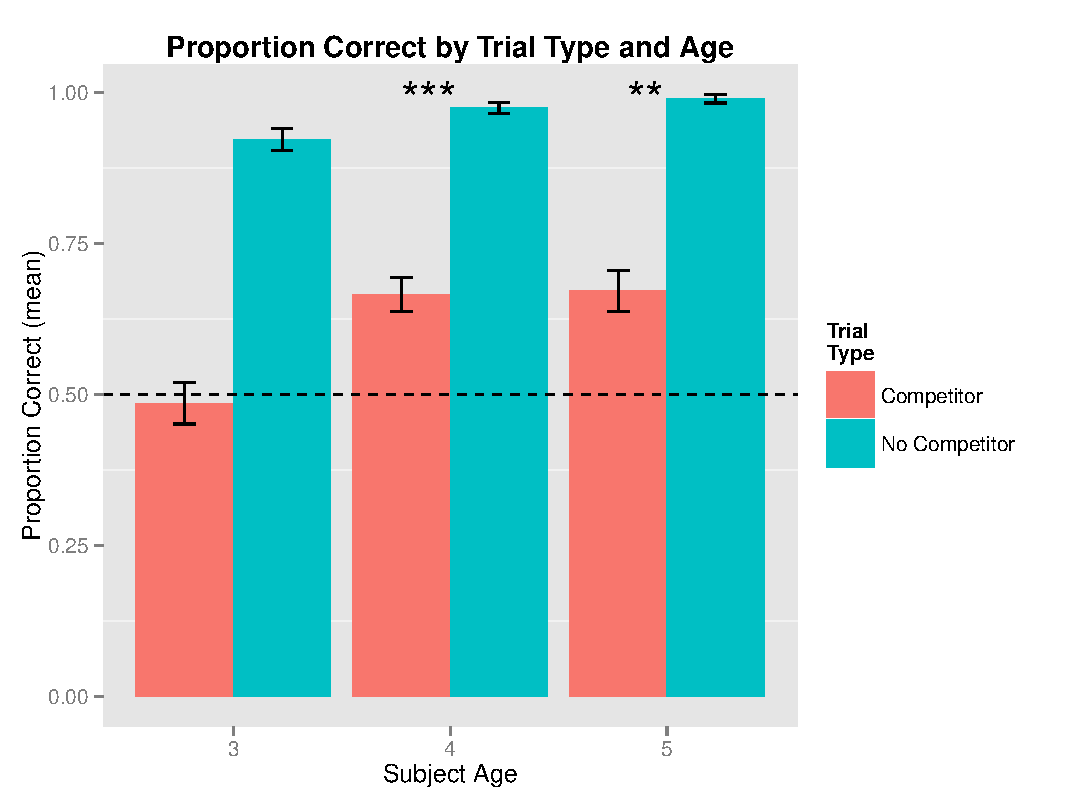
\includegraphics[scale=0.7]{CLAV_Exp1_ProportionCorrect.pdf}
\end{wrapfigure}
To quantify the reliability of these results, I fit a logistic mixed effects model (Gelman \& Hill, 2006; Jaeger, 2008; Quen� \& Van den Bergh, 2008) to children's responses, with age group and condition as fixed effects, and with random effects of condition fit for each participant and each target item (Barr, Levy, Scheepers, \& Tily, 2013; Baayen, Davidson, \& Bates, 2008). The resulting coefficient estimates suggested that three-year-olds (the reference level) were not above chance in their responding on critical trials ($\beta=-0.24$, $SE=0.29$, $z=-0.819$, $p=0.413$). There was a significant coefficient indicating higher performance on filler trials ($\beta=3.22$, $SE=0.31$, $z=10.336$, $p < 0.001$). There were significant coefficients for the effect of age, suggesting that both four-year-olds ($\beta=0.79$, $SE=0.18$, $z=2.794$, $p < 0.01$) and five-year-olds ($\beta=1.10$, $SE=0.32$, $z=3.406$, $p < 0.001$) were above chance in their responses on critical trials, though five-year-olds were not significantly more accurate than four-year-olds ($\beta=0.31$, $SE=0.30$, $z=1.031$, $p = 0.3$).\\ 

There was also a significant coefficient for the effect of gender ($\beta=0.76$, $SE=0.24$, $z=3.101$, $p = 0.002$), suggesting that female children performed significantly more accurately than male children. \begin{wrapfigure}{l}{0.7\linewidth}
	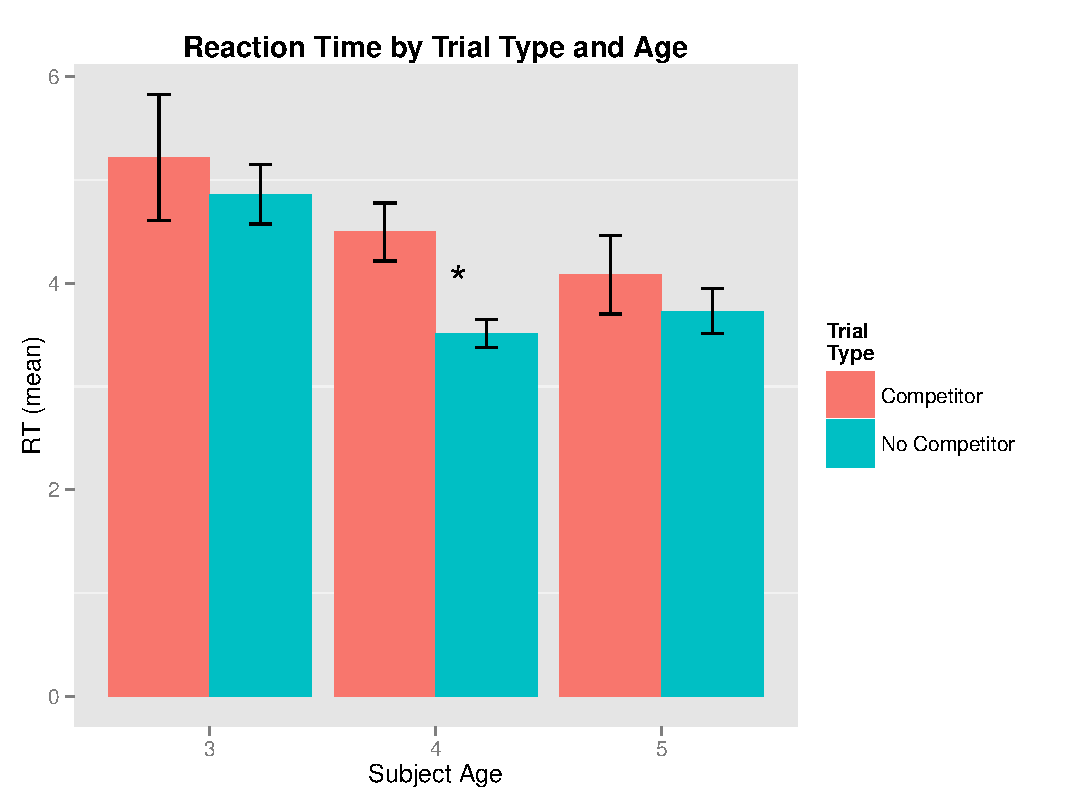
\includegraphics[scale=0.67]{CLAV_Exp1_MeanRT.pdf}
\end{wrapfigure}\\We see that during competitor trials, girls choose the correct-label, gender-consistent item during $66.4\%$ of trials, while males only select the correct-label, gender-consistent item $56.2\%$ of the time (for girls, $SD=47.2\%$, and for boys, $SD=49.7\%$). A model with a coefficient for gender provided significantly better fit to the data, ($\chi^2_1 = 9.37$, $p = 0.0002$), whereas a model with an age by gender interaction did not ($\chi^2_2 = 0.55$, $p = 0.759$).\\
\\
\\
\section{Discussion}
\subsection{Discussion of Results}
The results of Experiment 1 are consistent with the view that preschool-aged children do indeed use talker information in voice, map that information to developing forms of social categories, namely ideas and stereotypes about speaker gender, and can access and use this information to guide their interpretations and comprehension in situations where speaker meaning is ambiguous. These data also suggest a developmental trajectory for children's navigation of this process, as children are significantly above chance in their inference of a speaker preferring the object consistent with social gender stereotypes at age four, but at the age of three remain at or below chance. These results raise two important questions: First, why do three-year-olds struggle with the task when four-year-olds do not? Second, how might we interpret the significant effect of gender as a predictor of children's performance in the task?\\

As for the first question, by the nature of the task, there are several steps along the way to completing it at which children�s performance might break down. For instance, given that 3-year-olds choose one of the correct-label objects but are agnostic as to whether or not it is gender-consistent, it is first possible that 3-year-olds do not discriminate the gender of the speaker. Recall, however, that children as young as 6 months can discriminate the gender of a speaker based on speaker voice alone (Miller, 1983), so it is unlikely that the 3-year-olds are not correctly determining the gender of the speaker by their voice. 

Or perhaps children have yet to be able to map the gender of the speaker to their representational social knowledge and stereotypes about gender, which would imply that their use of talker information during speech perception is poor at this age.  As mentioned before, it is unlikely that the 3-year-olds are not correctly determining the gender of the speaker by their voice. Furthermore, children as young as 3 have been shown to be able to use acoustic cues to talker identity to activate their knowledge about the speaker and to constrain that speaker's domain of reference when the speaker is referring to him- or herself (Creel, 2012). It is unlikely then that children at age 3 are unable to make a mapping between speaker identity as determined by their voice and their knowledge about the person speaking. 

It could also be that children do not have access to representational social knowledge and stereotypes about gender, or that they do have access to it but do not think it is informative in this task. There is a consistent body of extensive survey data on American media consumption to suggest that children are at least exposed to these stereotypes by age three (Rideout et al., 2003, 2006), and four-year-olds� successful completion of the task coupled with past research on children�s understanding of register implies that even if the influence of this information is not yet strong enough to influence children�s behavior, it soon will be (Andersen, 1990).  
\begin{figure}[ht]
\centering
	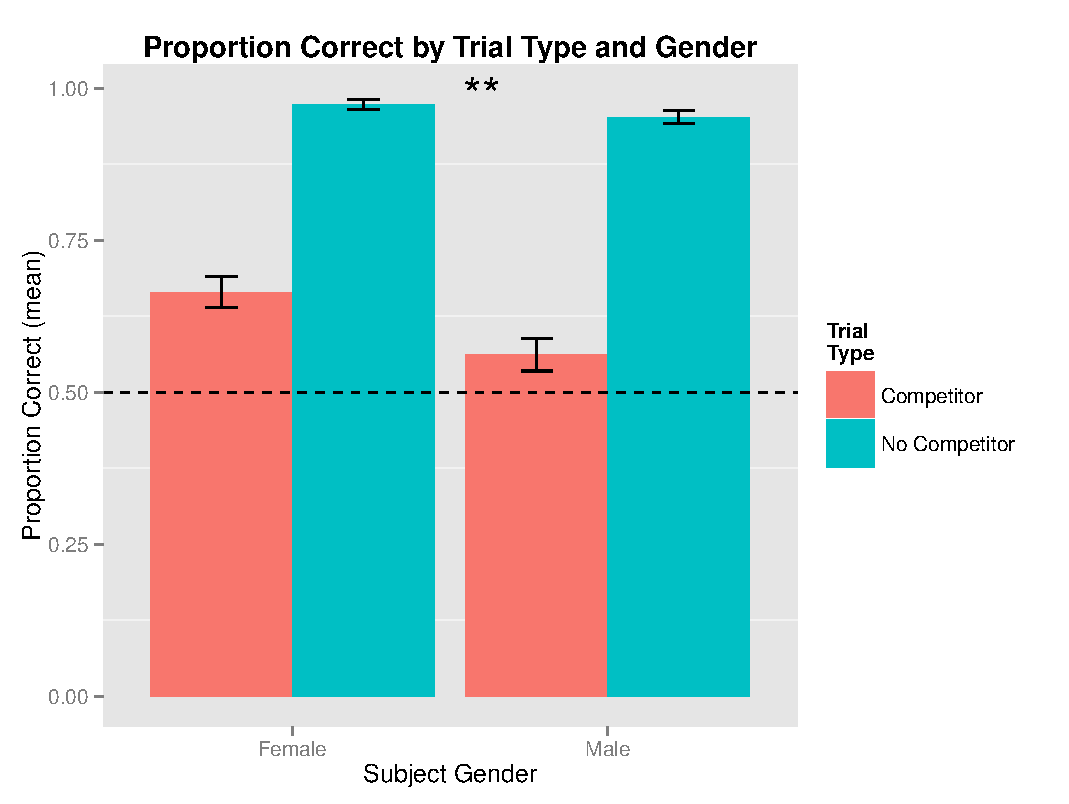
\includegraphics[scale=0.75]{CLAV_Exp1_Gender.pdf}
\end{figure}

Finally, perhaps children do not discriminate the gendered valence of the correct-label items. While this is possible, the fact that four-year-olds can succeed in the task, coupled with the strength of the difference scores for the pairs of correct-label items in the image-norming task on Mechanical Turk at least cast some doubt on this interpretation. However, it is not unreasonable to think that while 3-year-old children may have access to stereotype and representational information about gender, the differentiation of the correct-label items, while strong enough for adult judges, is not sufficiently strong enough for children of this age to see their difference as meaningful given their limited experience.

This remaining possibility would imply that these children are mapping speaker identity to their knowledge about social categories such as gender, but that their knowledge about these categories is not developed enough to allow them to infer the speaker�s intention based on their gender, at least not with respect to the items presented to them. 

In order to fully appreciate the discrimination that the 4-year-old children can currently make in this task, I turn briefly to a consideration of how gender information manifests itself in voice.

\subsection{Speaker Gender As Conveyed Through Voice}
A speaker's gender is a highly complex social construction that correlates with many linguistic variables, and it should be noted that multifaceted socially-influenced stylistic variation can still exist within gender groups, despite these correlations (Eckert, 1990). 

While gender is a construct that influences many aspects of human behavior, what aspects of people's voices convey social information such as gender? That males and females differ in their acoustic productions is well-known, with early experiments demonstrating significant differences in fundamental frequency and in formant structure between male and female speakers (Peterson \& Barney, 1952). Much of this difference though is likely due to the fact that gender is performed. Differentiation of voice characteristics along a gendered dimension appears quite early in development, with children's voices first differing by gender with respect to vowel formant frequencies (but not $f_0$) at the age of four, and then differing with respect to both vowel formant frequencies and fundamental frequency by the age of twelve. Even so, adults are able to reliably distinguish whether four-year-old children are male or female based only on their voice (Perry, et al., 2001).

Although the ways in which speakers perform gender is largely idiosyncratic to specific speech communities (Johnson, 2006), the sociophonetic individual listeners across speech communities and dialects maintain expectations and guidelines about how men and women are likely to talk in accordance with their gender (Podesva et al., 2015; Eckert, 1990, 2008;). Accordingly, there is a social component to the realization of gender in voice, leading to voice differences between different genders of speakers that are larger than might be expected if this difference were due to biological factors alone (Johnson, 2005). That is, speakers perform gender in line with their community's expectations for how males and females should talk (Johnson, 2005, 2006).  Evidence from previous studies suggests that these expectations are quite robust, with adults being able to correctly categorize voices as male or female even when acoustic correlates of gender such as fundamental frequency have been reduced or removed altogether (Fellowes, et al., 1997). Listeners can still be convinced of a speaker's gender, even when their speech signal is ambiguous or not strongly stereotyped (Johnson, 2006). Expectations about speaker gender and speaker voice will cause listeners to adjust their online interpretation of a speaker's utterances (Johnson, 1989), even leading adults to perceive the same word differently if they are told it is spoken by a man as opposed to a woman. For example, in some communities the acoustic boundary between the vowels in {\it hood} and in {\it hud} are different for male and female speakers (Johnson, 2005). Listeners also adjust their expectations about fricative duration and frequency for speakers of different genders in accordance with gender stereotypes that exist in their communities (Strand \& Johnson, 1996). Accordingly, listeners see a processing benefit when speaker voice is in line with their community's guidelines and expectations for performance of gender, and see a corresponding detriment when speaker voices are ambiguous with respect to gender or are in violation of the stereotypes prescribing proper male and female acoustic phonetic behavior (Strand 1999). These data suggest a powerful role for gender in conveying identity. This can be seen in other modalities as well, as adults struggle to ignore identity information while attempting a visual sex categorization task (Bulthoff, 2009), and adults have been shown to categorize faces more accurately and more quickly by sex than by race (Contreras et al., 2013).

All of this evidence points to the strength of speaker gender as an acoustic variable, and a substantial source of social meaning that even children can recognize from an early age.
 
\subsection{Implications for Children's Socialization}
Although this experimental paradigm was developed to examine young children's ability to utilize phonetically-cued social information in voice, a paradigm such as this one also acts as a measurement of how children are actually constructing gender stereotypes and social categories more broadly, and could conceivably be expanded to test children's intuitions about which variants of an object are more likely to belong to an adult speaker as opposed to a child.

I have argued that children's performance on this task reveals a robust understanding of gender stereotypes and thorough socialization by age 4. Prior work has for some time argued that socialization practices may be responsible for differences in male and female preschool competence (Baumrind \& Black, 1967); might this be at work in the gender difference I find in this experiment?

Past work on young children's socialization has found that gender and sex-role socialization is particularly focused on female preschoolers (Fagot \& Patterson, 1969; Weitzman, Eifler, Hokada, \& Ross, 1972). This work has found that it is often the case that teachers consistently reinforce feminine behaviors more than masculine behaviors, that girls are not affirmed by teachers when they perform opposite-sex behaviors but that boys are, and that by 3 years of age, there are sex differences in children's play behavior, and that same-sex peers reinforce this gendered behavior (Fagot \& Patterson, 1969). Yet other work has demonstrated that children's books and other forms of children's entertainment heavily reinforce to girls what feminine behavior ought to look like (Weitzman, et al., 1972). Therefore it should not come as a surprise that girls outperform boys on the critical trials, where children have to recognize the phonetically-cued social information in voice related to gender, recognize the gendered differences in the appearance of the two correct-label items, and use their knowledge of social stereotypes to align the speaker's gender to their supposed preference for the stereotype-consistent item.

\subsection{Future Directions}
Ongoing or future work could attempt to manipulate the visual features of the image stimuli used in an experimental paradigm such as this one to examine which precise features (color, shape, apparent texture, etc.) best cue gender to children observers. Doing so would provide valuable insight into the sheer extent of the socialization that children have received within their first five years of life as it would point to the visual features that preschool-aged children have already been taught to treat as masculine or feminine.

Ongoing or future work could also incorporate other social dimensions into this paradigm in order to examine the socialization children have received by the preschool years. Although I propose above examining children's performance on a version of this task with a child speaker and an adult speaker, the social dimensions that this paradigm could examine are not limited to age and gender.

The use of eyetracking in future studies would allow researchers to better investigate precisely why children who do not select the stereotype-consistent item in the correct-label pair do so, as their eyes' saccades and fixations would help to indicate whether they oscillate between the two correct-label choices or whether they select the first correct-label item they attend to (Nordmeyer \& Frank, 2014).
\section{Acknowledgements}
This work was supported by a Major Grant from Stanford Undergraduate Advising and Research. The author would like to thank Kevin B. McGowan, Meghan Sumner, and Michael C. Frank for their guidance and collaboration: thank you to Kevin B. McGowan for invaluable assistance in experimental design, creating and norming the images and image presentation, for optimizing the web experiment to ensure accurate reaction time measures, and for very helpful comments; thank you to both Meghan Sumner and Michael C. Frank for providing guidance in literature review, experimental design, analysis, and writeup critique. The author would also like to thank Eve V. Clark for her assistance in the analysis of relevant literature and for thorough and helpful comments, and the author would like to thank Masoud Jasbi and Ann Nordmeyer for helpful comments, advice, and support.
\section{References}
\begin{enumerate}
\item Allen, J. S., Miller, J. L., \& DeSteno, D. (2003). Individual talker differences in voice-onset-time. {\it Journal of the Acoustical Society of America}, {\it 113}, 544-552.
\item Andersen, E. S. (1990). {\it Speaking with style: The sociolinguistic skills of children.} London: Routledge.
\item Andersen, E. S., \& Johnson, C. E. (1973). Modifications in the speech of an eight-year-old as a reflection of age of listener. {\it Stanford Occasional Papers in Linguistics}, 3, 149-160.
\item Andersen, E. (1979). Register variation in young children's role-play speech. In {\it Proceedings of the Society for Research in Child Development}.
\item Aubrey, J. S., \& Harrison, K. (2004). The gender-role content of children's favorite television programs and its links to their gender-related perceptions. {\it Media Psychology}, 6(2), 111-146.
\item Baayen, R. H., Davidson, D. J., \& Bates, D. M. (2008). Mixed-effects modeling with crossed random effects for subjects and items. {\it Journal of memory and language, 59(4)}, 390-412.
\item Bargh, J. A., Chen, M., \& Burrows, L. (1996). Automaticity of social behavior: Direct effects of trait construct and stereotype activation on action. {\it Journal of personality and social psychology, 71(2)}, 230.
\item Barr, D. J., Levy, R., Scheepers, C., \& Tily, H. J. (2013). Random effects structure for confirmatory hypothesis testing: Keep it maximal. {\it Journal of Memory and Language, 68(3)}, 255-278.
\item Baumrind, D., \& Black, A. E. (1967). Socialization practices associated with dimensions of competence in preschool boys and girls. {\it Child development}, 291-327.
\item Bellinger, D. C., \& Gleason, J. B. (1982). Sex differences in parental directives to young children. {\it Sex Roles}, 8(11), 1123-1139.
\item Bicknell, K., Elman, J. L., Hare, M., McRae, K., \& Kutas, M. (2008). Online expectations for verbal arguments conditional on event knowledge. {\it Proceedings of the 30th Annual Conference of the Cognitive Science Society} (pp. 2220-2225). Austin, TX: Cognitive Science Society.
\item Borovsky, A., \& Creel, S. C. (2014). Children and adults integrate talker and verb information in online processing. {\it Developmental psychology}, {\it 50(5)}, 1600.
\item Brouwer, D., \& de Haan, D. (1987). {\it Women's language, socialization and self-image (Vol. 4)}. Foris Publications.
\item B�lthoff I, (2009). Sex categorization is influenced by facial information about identity. {\it Perception}, {\it 38}, ECVP Abstract Supplement, 78.
\item Clark, H. H. (1996). {\it Using language}. Cambridge: Cambridge University Press.
\item Comstock, G., \& Scharrer, E. The Use of Television and Other Screen Media. in Singer, D. G., \& Singer, J. L. (Eds.). (2011). {\it Handbook of Children and the Media.} Sage publications.
\item Contreras, J. M., Banaji, M. R., \& Mitchell, J. P. (2013). Multivoxel patterns in fusiform face area differentiate faces by sex and race. {\it PloS one, 8(7)}, e69684.
\item Creel, S. C., Aslin, R. N., \& Tanenhaus, M. K. (2008). Heeding the voice of experience: The role of talker variation in lexical access. {\it Cognition}, {\it 108}, 633-664.
\item Creel, S. C., \& Tumlin, M. A. (2011). On-line acoustic and semantic interpretation of talker information. {\it Journal of Memory and Language}, {\it 65}, 264-285.
\item Creel, S. C. (2012). Preschoolers' Use of Talker Information in On-Line Comprehension. {\it Child development}, {\it 83}, 2042-2056.
\item Dahan, D., \& Tanenhaus, M. K. (2004). Continuous mapping from sound to meaning in spoken-language comprehension: immediate effects of verb-based thematic constraints. {\it Journal of Experimental Psychology: Learning, Memory, and Cognition}, {\it 30}, 498.
\item Eckert, P. (1989). The whole woman: Sex and gender differences in variation. {\it Language variation and change}, {\it 1(03)}, 245-267.
\item Eckert, P. (2008). Variation and the indexical field. {\it Journal of sociolinguistics}, {\it 12(4)}, 453-476.
\item Fagot, B. I., \& Patterson, G. R. (1969). An in vivo analysis of reinforcing contingencies for sex-role behaviors in the preschool child. {\it Developmental Psychology}, {\it 1(5)}, 563.
\item Fellowes, J. M., Remez, R. E., \& Rubin, P. E. (1997). Perceiving the sex and identity of a talker without natural vocal timbre. {\it Perception \& Psychophysics}, {\it 59}, 839-849.
\item Freeman, J. B., \& Ambady, N. (2011). A dynamic interactive theory of person construal. {\it Psychological review}, {\it 118(2)}, 247.
\item Gelman, A., \& Hill, J. (2006). {\it Data analysis using regression and multilevel/hierarchical models.} Cambridge University Press.
\item Gleason, J. B. (1973). Code Switching in Children's Language.  In Moore, T. (Ed.). {\it Cognitive Development and the Acquisition of Language (Academic Press)}. pp. 169-167.
\item Gleason, J. B. (1975). Fathers and Other Strangers: Men's speech to Young Children. {\it 26th Annual Georgetown University Roundtable (Georgetown University Press)}. pp. 289-97.
\item Goldinger, S. D. (1996). Words and voices: Episodic traces in spoken word identification and recognition memory. {\it Journal of Experimental Psychology: Learning, Memory, and Cognition}, {\it 22}, 1166-1183.
\item Goldinger, S. D. (1998). Echoes of echoes? An episodic theory of lexical access. {\it Psychological review}, {\it 105}, 251.
\item Greenwald, A. G., \& Banaji, M. R. (1995). Implicit social cognition: attitudes, self-esteem, and stereotypes. {\it Psychological review, 102(1),} 4.
\item Greif, E. B. (1980). Sex differences in parent-child conversations. {\it Women's Studies International Quarterly}, 3(2), 253-258.
\item Hanna, J. E., \& Tanenhaus, M. K. (2004). Pragmatic effects on reference resolution in a collaborative task: Evidence from eye movements. {\it Cognitive Science}, {\it 28}, 105-115.
\item Jaeger, T. F. (2008). Categorical data analysis: Away from ANOVAs (transformation or not) and towards logit mixed models. {\it Journal of memory and language}, {\it 59(4)}, 434-446.
\item Johnson, K. (1989) Higher formant normalization results from auditory integration of F2 and F3. {\it Perception and Psychophysics. 46}, 174-180.
\item Johnson, K. A., Strand, E. A., \& D'imperio, M. (1999). Auditory-visual integration of talker gender in vowel perception. {\it Journal of Phonetics}, {\it 24}, 359-384.
\item Johnson, K. A. (2005). Speaker normalization in speech perception. In D. B. Pisoni \& R. E. Remez (Eds.), {\it Handbook of speech perception} (pp. 363-389). Oxford: Blackwell.
\item Johnson, K. (2006). Resonance in an exemplar-based lexicon: The emergence of social identity and phonology. {\it Journal of phonetics}, {\it 34}, 485-499.
\item Kaganovich, N., Francis, A. L., \& Melara, R. D. (2006). Electrophysiological evidence for early interaction between talker and linguistic information during speech perception. {\it Brain research}, {\it 1114(1)}, 161-172.
\item Kempson, R. (2001). Pragmatics: Language and communication. In M. Aronoff \& J. Rees-Miller (Eds.), {\it Handbook of linguistics}. Malden, MA: Blackwell.
\item Ladefoged, P., \& Broadbent, D. E. (1957). Information conveyed by vowels. {\it The Journal of the Acoustical Society of America}, {\it 29}, 98-104.
\item Liberman, A. (1970). The grammars of speech and language. {\it Cognitive Psychology}, {\it 1}, 301-323.
\item Maccoby, E., \& Jacklin, C. (1974). {\it The Psychology of Sex Differences.} Stanford: Stanford University Press.
\item McGillicuddy-De Lisi, A. V. \& De Lisi, R. (Eds.). (2002). {\it Biology, Society, and Behavior: The Development of Sex Differences in Behavior.} Westport: Greenwood Publishing Group. Has even more gender stereotypes work and a variety of other perspectives on gender behavior.
\item Miller, C. L. (1983). Developmental changes in male/female voice classification by infants. {\it Infant Behavior and Development}, {\it 6}, 313-330.
\item Nordmeyer, A. E., \& Frank, M. C. (2014). The role of context in young children�s comprehension of negation. {\it Journal of Memory and Language}, {\it 77}, 25-39.
\item Nygaard, L. C., Sommers, M. S., \& Pisoni, D. B. (1994). Speech perception as a talker-contingent process. {\it Psychological Science}, {\it 5}, 42-46.
\item Nygaard, L. C. (2005). Perceptual integration of linguistic and non-linguistic properties of speech. In D. B. Pisoni \& R. E. Remez (Eds.), {\it Handbook of speech perception} (pp. 390-413). Oxford: Blackwell.
\item Rideout, V. J., Vandewater, E. A., \& Wartella, E. A. (2003). {\it Zero to six: electronic media in the lives of infants, toddlers and preschoolers}. Henry J. Kaiser Family Foundation.
\item Rideout, V., \& Hamel, E. (2006). {\it The media family: Electronic media in the lives of infants, toddlers, preschoolers and their parents.} Henry J. Kaiser Family Foundation.
\item Palmeri, T. J., Goldinger, S. D., \& Pisoni, D. B. (1993). Episodic encoding of voice attributes and recognition memory for spoken words. {\it Journal of Experimental Psychology: Learning, Memory, and Cognition}, {\it 19}, 309.
\item Patterson, M. L. \& Werker, J. F. (2002). Infants' ability to match dynamic phonetic and gender information in the face and voice. {\it Journal of Experimental Child Psychology}, {\it 81}, 93-115.
\item Perry, J. (1997). Indexicals and demonstratives. In C. Wright \& R. Hale (Eds.), {\it Companion to the philosophy of language} (pp. 586-612). Oxford: Blackwell.
\item Perry, T. L., Ohde, R. N., \& Ashmead, D. H. (2001). The acoustic bases for gender identification from children's voices. {\it The Journal of the Acoustical Society of America}, {\it 109}, 2988-2998.
\item Peterson, G. E., \& Barney, H. L. (1952). Control methods used in a study of the vowels. {\it The Journal of the Acoustical Society of America}, {\it 24}, 175-184.
\item Philips, S. U., Steele, S., \& Tanz, C. (Eds.). (1987). {\it Language, gender, and sex in comparative perspective} (No. 4). Cambridge University Press.
\item Podesva, R. J., Reynolds, J., Callier, P., \& Baptiste, J. (2015). Constraints on the social meaning of released {\it /t}: A production and perception study of US politicians. {\it Language Variation and Change}, {\it 27(01)}, 59-87.
\item Quen�, H., \& Van den Bergh, H. (2008). Examples of mixed-effects modeling with crossed random effects and with binomial data. {\it Journal of Memory and Language, 59(4)}, 413-425.
\item Remez, R. E., Fellowes, J. M., \& Rubin, P. E. (1997). Talker identification based on phonetic information. {\it Journal of Experimental Psychology: Human Perception and Performance}, {\it 23}, 651.
\item Rideout, V. J., Vandewater, E. A., \& Wartella, E. A. (2003). {\it Zero to six: electronic media in the lives of infants, toddlers and preschoolers}. Henry J. Kaiser Family Foundation.
\item Rideout, V., \& Hamel, E. (2006). {\it The media family: Electronic media in the lives of infants, toddlers, preschoolers and their parents.} Henry J. Kaiser Family Foundation.
\item Sachs, J. (1987). Preschool boys' and girls' language use in pretend play. {\it Language, gender, and sex in comparative perspective}, 178-188.
\item Sumner, Meghan. (2015). The social weight of spoken words. {\it Trends in Cognitive Sciences},{\it 19(5)}, 238 - 239.
\item Sumner, M., Kim, S. K., King, E. \& McGowan K. B. (2014). The socially weighted encoding of spoken words: a dual-route approach to speech perception. {\it Frontiers in psychology}, 4.
\item Strand, E A. \& Johnson, K. (1996). Gradient and visual speaker normalization in the perception of fricatives. In Dafydd Gibbon (Ed.), {\it Natural Language Processing and Speech Technology: Results of the 3rd KONVENS Conference, Bielefeld, October 1996}, (pp. 14-26). Berlin, Germany: Mouton de Gruyter.
\item Strand, E.A. (1999). Uncovering the role of gender stereotypes in speech perception. {\it Journal of Language and Social Psychology}, {\it 18:1}, 86-100.
\item Strand, E. A. (2000). Gender stereotype effects in speech processing (Doctoral dissertation, {\it The Ohio State University}).
\item Van Berkum, J. J., van den Brink, D., Tesink, C. M., Kos, M., \& Hagoort, P. (2008). The neural integration of speaker and message. {\it Journal of Cognitive Neuroscience}, {\it 20}, 580-591.
\item Wild, H., Barrett, S., Spence, M. J., O'Toole, A. J., Cheng, Y. D., \& Brooke, J. (2000). Recognition and Sex Categorization of Adults' and Children's Faces: Examining Performance in the Absence of Sex-Stereotyped Cues. {\it Journal of Experimental Child Psychology}, {\it 77}, 269-291.
\item Weitzman, L. J., Eifler, D., Hokada, E., \& Ross, C. (1972). Sex-role socialization in picture books for preschool children. {\it American journal of Sociology}, 1125-1150.
\end{enumerate}
\end{document}